\section{Motor}
The motor controller is based on a simple driver interface. The ports and generics are described in the table underneath. 
The driver is written for the L6203 Full Bridge driver. The bridge is active low, so is the designed component, besides that
the Full Bridge supports up to 100KHz, higher switching freq is not recommended.

\begin{tabular}{|c|p{7.5cm}|}
\hline 
Generics & Description\tabularnewline
\hline 
\hline 
pwm\_max\_valu : integer := 128 & This is the counter value. The motor is using phase correct PWM. \tabularnewline
\hline 
pwm\_freq : integer := 10000 & This is the motor frequency, based on intern clk division.\tabularnewline
\hline 
\hline 
Ports & Description\tabularnewline
\hline 
\hline 
stop\_btn : in std\_logic & An emergency button. An emergency button. When set high motor stops on next ready rising edge.\tabularnewline
\hline 
ready : in std\_logic & A message from top module, activated on rising edge.\tabularnewline
\hline 
clk : in std\_logic; & Internal clk from FPGA is parsed to generate clk for the motor.\tabularnewline
\hline 
pwm\_set : in std\_logic\_vector(6 downto 0); & Set the motor speed on next ready.\tabularnewline
\hline 
direction : in std\_logic; & Set the direction of the motor on next ready, 1 is forward/right - 0 backwards/left.\tabularnewline
\hline 
motor\_o : out std\_logic\_vector(1 downto 0); & Two motor outputs for the H-bridge. LSB is forward/right, MSB is
backwards/left.\tabularnewline
\hline 
chip\_enable : out std\_logic; & Enable the H-bridge.\tabularnewline
\hline 
\end{tabular}

\subsection{Motor Connection}
A quick guide to the pins, IN1 is for MOTOR1, it has 3 different pins: A is used for right/forward, B is used left/backward and enable pins inorder for it to function. GND is ground and VCC is 12V from source. More to come....

\begin{figure}[H]
    \centering
    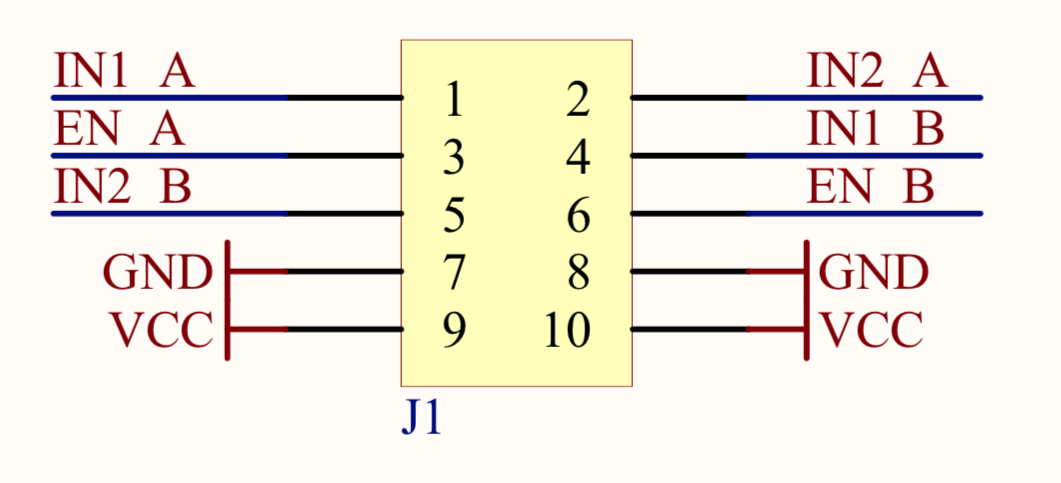
\includegraphics[width=\textwidth]{assets/img/H_bridge_pinout.png}
    \caption{motor pins}
    \label{fig:mcu_architecture}
\end{figure}


%%%\end{document}